Brechung tritt auf, wenn ein Lichtstrahl nichtsenkrecht von einem Medium auf ein anderes fällt. Die Änderung des Winkels, die beim Auftreffen auf die Grenzfläche erfolgt, wird Brechung genannt. Diese Richtungsänderung des Lichstrahls wird durch die Wechselwirkung des elektrischen Feldes der Lichtwelle mit den Elektronen und Ionenrümpfen in der Materie verursacht.
Dies erklärt auch, warum die Ausbreitungsgeschwindigkeit von Licht in Materie $(v)$ kleiner ist, als die im Vakuum $(c)$, was im Verlauf des Kapitels noch ausführlicher erläutert wird.
Licht weist in verschiedenen Materialien unterschiedliche Ausbreitungsgeschwindigkeiten auf und das Verhältnis zwischen zweier solcher Geschwindigkeiten definiert den Brechungsindex $n$

\begin{equation}
  n := \frac{v_1}{v_2} \; ,
  \label{equ:n}
\end{equation}

welcher die Brechung als physikalische Größe beschreibt. Vergleicht man die Ausbreitungsgeschwindigkeit von Licht in einem Medium mit der im Vakuum $(v_1 = c)$, erhält man also den Faktor, um welchen die Phasengeschwindigkeit und
die Wellenlänge des Lichts beim Übergang in das Medium kleiner geworden ist. Medien mit höherem Brechungsindex als das Vergleichsmedium werden daher \emph{optisch dichter} genannt.

\subsection{Snelliussches Brechungsgesetz}
Der Brechungsindex eines Mediums wird in der Optik allerdings nicht über die
Ausbreitungsgeschwindigkeiten bestimmt, sondern mit Hilfe des Eintritts- und
Austrittswinkels (gemessen an der Normalen der Grenzfläche). Der Zusammenhang wird mit dem \emph{Huygensschen Prinzip} erklärt. Das Prinzip besagt, dass jeder Punkt einer Wellenfront als Ursprung einer kugelförmigen \emph{Elementarwelle} betrachtet werden kann und damit die Wellenfront für jeden späteren Zeitpunkt durch die Einhüllende von allen einzelnen Elementarwellen bestimmt ist.
Dafür werden zwei parallele Lichtstrahlen betrachtet die mit einem Winkel $\alpha$
auf die Grenzfläche des Mediums auftreffen und daraufhin in einem Winkel $\beta$ in das Medium eindringen (siehe Abbildung \ref{fig:SBG}).

\begin{figure}
  \centering
  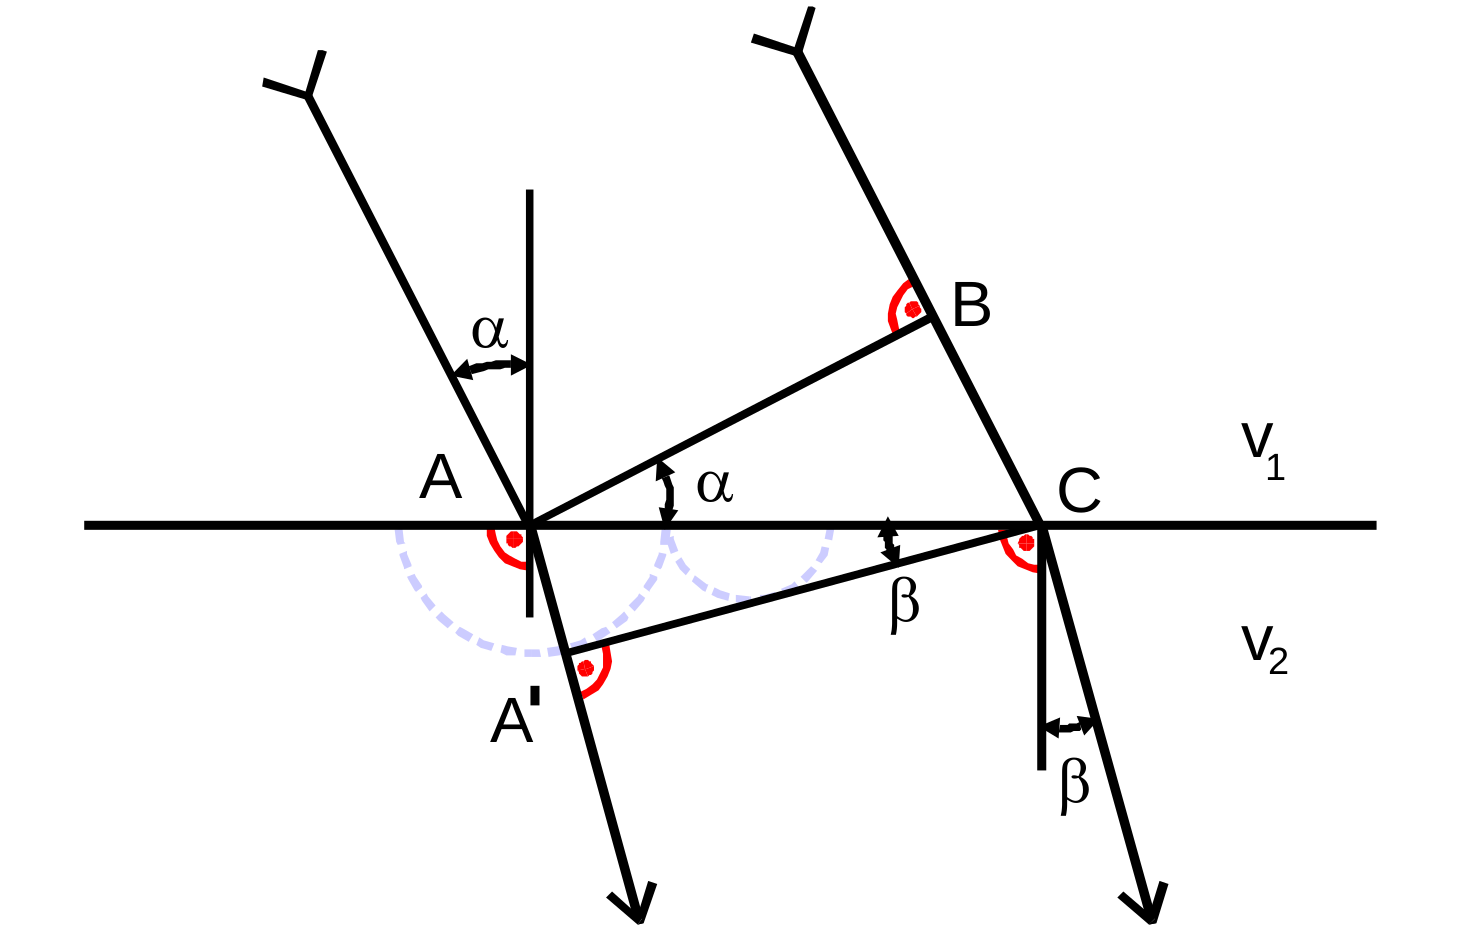
\includegraphics[width=0.6\textheight]{../figures/SBG.png}
  \caption{Veranschaulichung des Strahlengangs mit Hilfe des Huygensschen Prinzips. [Skript V402]}
\label{fig:SBG}
\end{figure}

Wie in Abbildung \ref{fig:SBG} zu sehen ist, trifft die ebene Wellenfront $(\overline{AB})$ im Punkt A schneller auf die Grenzfläche, als im Punkt C. In dieser Zeit $(t_1 = \overline{BC} / v_1)$ hat die Elementarwelle die im Punkt A entsteht, sich schon um $r = t_1v_2$ ausgebreitet, während die im Punkt C erst entsteht.
Durch geometrische Überlegungen lässt sich nun die Beziehung

\begin{equation}
  \frac{\sin{\alpha}}{\sin{\beta}} = \frac{v_1}{v_2} = n
\end{equation}

herleiten, die als \emph{Snelliussches Brechungsgesetz} bekannt ist.

\subsection{Ableitung der Dispersionsrelation}
Dispersion ist ein Phänomen, welches die Frequenzabhängigkeit einer physikalischen Größe beschreibt, in der Optik handelt es sich dabei um die Ausbreitungsgeschwindigkeit von Licht in einem Medium. Nach Gleichung \eqref{equ:n} ist somit auch der Brechungsindex eine frequenzabhängige Größe bzw. abhängig von der Wellenlänge $\lambda$ des Lichtes
\begin{equation}
    n = f(\lambda) \; .
\end{equation}
Dabei handelt es sich um die Dispersionsgleichung, die sich aus der Maxwellschen Theorie elektromagnetischer Wellen ergibt. Dies lässt sich allerdings nur anwenden, wenn die Materie nicht mehr als Kontinuum betrachtet wird, sondern als Ansammlung elektrisch geladener Teilchen, wie Elektronen und Ionenrümpfe. Die Ionenrümpfe können aber für diese Betrachtung vernachlässigt werden, da sichtbares Licht betrachtet wird und diese Wechselwirkung erst bei größeren Wellenlängen eine signifikante Auswirkung hat.

Trifft Licht auf Materie werden die Elektronen durch das elektrische Feld
der Lichtwelle aus ihrer Gleichgewichtslage ausgelenkt. Durch das Wechselfeld wirkt daher eine periodische Kraft auf die Ladungen und führt zu einer erwzungenen Schwingung. Dabei treten auch Resonanzerscheinungen auf, an denen die Materie erkennbar Energie der Lichtwelle absorbiert. Diese klassische Betrachtungsweise reicht aber nicht vollkommen aus um die Wechselwirkung von Licht mit Materie zu beschreiben, dafür wird die Quantentheorie benötigt. Um das zu vermeiden werden in diesem Versuch nur Wellenlängen betrachtet, die genug von den Resonanzstellen entfernt sind, damit die Absorption vernachlässigbar klein wird. Das ist zum Beispiel bei sichtbarem Licht das auf Glas trifft gegeben.

Das Magnetfeld der Lichtwelle erzeugt eine Lorentzkraft, welche die geladenen Teilchen aus ihrer Gleichgewichtslage verschiebt und damit einen elektrischen Dipol erzeugt. Die Polarisation des Mediums ist durch
\begin{equation}
  \vec P = \sum_{h} \vec P_h = \sum_{h} N_h q_h \vec x_h
  \label{equ:P}
\end{equation}
gegeben, mit den Ladungsträgern $q_h$, der Anzahl dieser Ladungsträger pro Volumeneinheit $N_h$, der Auslenkung aus der Gleichgewichtslage $\vec x_h$, während $h$ die unterschiedlichen Teilchenarten bezeichnet.

Eine Auslenkung aus der Gleichgewichtslage erzeugt eine dazu proportionale rücktreibende Kraft. Hinzu kommt eine Dämpfung auf Grund der periodischen Bewegung im elektromagnetischen Feld, die als \emph{"Reibungskraft"} proportional zur Geschwindigkeit der Teilchen sein soll.

Für die Bewegung der Teilchen ergibt sich daraus eine Differentialgleichung der Art
\begin{equation}
  m_h \frac{\mathrm d^2 \vec{x_h}}{\mathrm dt^2} + f_h \frac{\mathrm d \vec{x_h}}{\mathrm dt } + a_h \vec{x_h} = q_h \vec E_0 e^{i \omega t}
  \label{equ:DGL}
\end{equation}
mit den Ladungsträgern $q_h$ und der Teilchenmasse $m_h$. Die Lösung einer solchen Differentialgleichung ist bekannt. Mit Hilfe der Polarisation aus Gleichung \eqref{equ:P} und der \emph{Maxwellschen Relation}
\begin{equation}
  n^2 = \epsilon
  \label{equ:MaxwellRel}
\end{equation}
ergibt sich nach einigen Umformungsschritten der gesuchte Ausdruck für den Brechungsindex in Abhängigkeit der Frequenz des Lichts
\begin{equation}
  \tilde n^2 = 1 + \sum_{h} \frac{1}{\omega_h^2 - \omega^2 + \mathrm{i}\omega \frac{f_h}{m_h}}\frac{N_h q_h^2}{m_h \epsilon_0} \; .
  \label{equ:nkomplex}
\end{equation}
Der Brechungsindex $\tilde n$ ist komplex und kann folglich als
\begin{equation}
  \tilde n = n (1 - \mathrm{i}k)
  \label{equ:nkomplex2}
\end{equation}
mit dem in Gleichung \eqref{equ:n} beschriebenen reellen Brechungsindex $n$ und der Absorptionskonstanten $k$ geschrieben werden. Für die Brechung ist vor allem der Realteil von $\tilde n$ von Interesse. Da die Betrachtung ausreichend weit von den Resonanzstellen entfernt sein soll, wird die Aborption vernachlässigbar klein und damit ist
\begin{equation}
  n^2k \approx 0 \; .
  \label{equ:Naeherung}
\end{equation}
Anschaulich ist die betrachtete Materie damit praktisch farblos und durchsichtig bei den beobachteten Wellenlängen.
Da die Frequenz $\omega$ nicht gemessen werden kann, wird sie durch die Wellenlänge im Vakuum $\lambda$ ersetzt. Daraus ergibt sich für den Brechungsindex
\begin{equation}
  n^2(\lambda) = 1 + \sum_h \frac{N_h q_h^2}{4 \pi^2 c^2 \epsilon_0 m_h}\frac{\lambda^2\lambda_h^2}{\lambda^2 - \lambda_h^2} \; .
  \label{equ:nlambda}
\end{equation}

An dieser Stelle ist nun eine Fallunterscheidung notwendig: Es wird davon ausgegangen, dass das Medium nur eine Absorptionsstelle $\lambda_1$ besitzt. Dann muss zwischen Wellenlängen unterschieden werden, die entweder sehr viel größer oder sehr viel kleiner als $\lambda_1$ sind.

\subsubsection{Wellenlänge $\lambda \gg \lambda_1$}
Werden nur Wellenlängen $\lambda \gg \lambda_1$ betrachtet, kann eine Reihenentwicklung von Gleichung~\eqref{equ:nlambda} nach Potenzen von $\lambda_1/\lambda$ durchgeführt werden. Daraus ergibt sich für den Brechungsindex
\begin{equation}
  n^2(\lambda) = 1 + \frac{N_1 q_1^2 \lambda_1^2}{4 \pi^2 c^2 \epsilon_0 m_1} (1 + (\frac{\lambda_1}{\lambda})^2 + (\frac{\lambda_1}{\lambda})^4 + \cdots )
  \label{equ:taylor1}
\end{equation}
bzw. die \emph{Cauchysche Dispersionsformel}
\begin{align}
  n^2(\lambda) = A_0 + \frac{A_2}{\lambda^2} + \frac{A_4}{\lambda^4} + \cdots
  \label{equ:cauchy}
  \shortintertext{mit}
  A_0, A_2, A_4 > 0 \; .
\end{align}

Der Kurvenverlauf von Gleichung~\eqref{equ:cauchy} ist in Abbildung~\ref{fig:disper1} dargestellt.

\begin{figure}
  \centering
  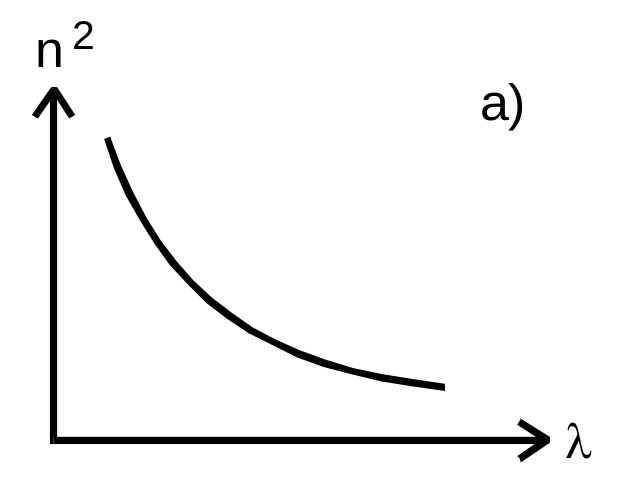
\includegraphics[width=0.4\textheight]{../figures/disper1.png}
  \caption{Dispersionskurve nach der Cauchyschen Dispersionsformel $(\lambda \gg \lambda_1)$. [Skript V402]}
\label{fig:disper1}
\end{figure}

\subsubsection{Wellenlänge $\lambda \ll \lambda_1$}
Jetzt werden Wellenlängen mit $\lambda \ll \lambda_1$ betrachtet, die Reihenentwicklung von Gleichung~\eqref{equ:nlambda} ergibt
\begin{equation}
  n^2(\lambda) = 1 - \frac{N_1 q_1^2 }{4 \pi^2 c^2 \epsilon_0 m_1} (\lambda^2 + (\frac{\lambda^4}{\lambda_1^2}) + (\frac{\lambda^6}{\lambda_1^4}) + \cdots )
  \label{equ:taylor2}
\end{equation}
bzw.
\begin{align}
  n^2(\lambda) = A_0 - A_2'\lambda^2 - A_4'\lambda^4 - \cdots
  \label{equ:disper2}
  \shortintertext{mit}
  A_i' > 0 \text{ für } \mathrm{i} \ge 2 \; .
\end{align}

Die grafische Darstellung des Kurvenverlaufs aus Gleichung~\eqref{equ:disper2} ist in Abbildung~\ref{fig:disper2} dargestellt.

\begin{figure}
  \centering
  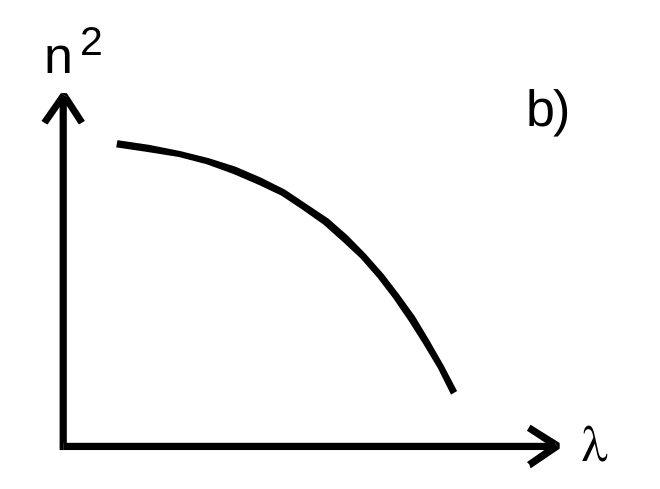
\includegraphics[width=0.4\textheight]{../figures/disper2.png}
  \caption{Dispersionskurve nach Gleichung~\eqref{equ:disper2} mit $\lambda \ll \lambda_1$. [Skript V402]}
\label{fig:disper2}
\end{figure}


Für beide Fälle ergeben sich demnach unterschiedliche Kurvenverläufe (mit unterschiedlicher Krümmung -- zu sehen in Abbildung~\ref{fig:disper1} und \ref{fig:disper2} ), aber in beiden Kurven nimmt der Brechungsindex mit zunehmender Wellenlänge ab (\emph{normale Dispersion}). Um herauszufinden, welche Dispersiongleichung das Material am besten beschreibt, werden einfach die Messdaten mit den Kurvenverläufen verglichen.






%the end
